%%%%%%%%%%%%%%%%%%%%%%%%%%%%%%%%%%%%%%%%%%%%%%%%%%%%%%%%%%%%%%%%%%%%%%%%%%%%%%%%%%
\begin{frame}[fragile]\frametitle{}
\begin{center}
{\Large Introduction to LangChain}
\end{center}
\end{frame}

% %%%%%%%%%%%%%%%%%%%%%%%%%%%%%%%%%%%%%%%%%%%%%%%%%%%%%%%%%%%%%%%%%%%%%%%%%%%%%%%%%%
% \begin{frame}[fragile]\frametitle{Introduction to LangChain}

% Agenda:
% \begin{itemize}
    % \item Library installation
    % \item Obtaining OpenAI credentials
    % \item Generating predictions using a language model
    % \item Constructing chains
    % \item Incorporating memory
    % \item Utilizing vector databases
    % \item Using Deep Lake as vector store (with a practical example)
    % \item Tools and agents: Vector store Agent
    % \item Combining tools with appropriate agents
    % \item Initiating and managing agents as orchestrators
% \end{itemize}

% \end{frame}

%%%%%%%%%%%%%%%%%%%%%%%%%%%%%%%%%%%%%%%%%%%%%%%%%%%%%%%%%%%%%%%%%%%%%%%%%%%%%%%%%%
\begin{frame}[fragile]\frametitle{What is LangChain?}

\textbf{LangChain}: {\bf Lang} stands for {\bf language} and {\bf chain} for connecting tasks


{\tiny (Ref: LangChain 101: Part 1. Building Simple Q\&A App - Ivan Reznikov)}

\begin{lstlisting}
+==========+========================+====================+====================+
|          | LangChain              | LLM                | ChatGPT            | 
+==========+========================+====================+====================+
| Type     | Framework              | Model              | Model              | 
+----------+------------------------+--------------------+--------------------+
| Purpose  | Build applications     | Generate text      | Generate chat      | 
|          | with LLMs              |                    | conversations      | 
+----------+------------------------+--------------------+--------------------+
| Features | Chains, prompts, LLMs, | Large dataset of   | Large dataset of   | 
|          | memory, index, agents  | text and code      | chat conversations | 
+----------+------------------------+--------------------+--------------------+
| Pros     | Can combine LLMs with  | Generates nearly   | Generates realistic| 
|          | programming techniques | human-quality text | chat conversations | 
+----------+------------------------+--------------------+--------------------+
| Cons     | Requires some          | Not as easy to use | Not as versatile   | 
|          | programming knowledge  | for specific tasks | as LangChain       | 
+----------+------------------------+--------------------+--------------------+
\end{lstlisting}
\end{frame}


%%%%%%%%%%%%%%%%%%%%%%%%%%%%%%%%%%%%%%%%%%%%%%%%%%%%%%%%%%%%%%%%%%%%%%%%%%%%%%%%%%
\begin{frame}[fragile]\frametitle{What is LangChain?}

Framework built to help you build LLM-powered applications more easily by providing 

\begin{itemize}
\item a generic interface to a variety of different foundation models,
\item a framework to help you manage your prompts 
\item a central interface to long-term memory , external data , other LLMs , and other agents for tasks an LLM is not able to handle (e.g., calculations or search).
\end{itemize}

It is an open-source project (https://github.com/hwchase17/langchain) created by Harrison Chase.

{\tiny (Ref: Getting Started with LangChain: A Beginner’s Guide to Building LLM-Powered Applications by Leonie Monigatti)}
\end{frame}



%%%%%%%%%%%%%%%%%%%%%%%%%%%%%%%%%%%%%%%%%%%%%%%%%%%%%%%%%%%%%%%%%%%%%%%%%%%%%%%%%%
\begin{frame}\frametitle{What is LangChain?}

\begin{itemize}
\item LangChain Open source platform to be used to work with Large Language Models (LLMs). 
\item Integrates will many popular LLM providers like OpenAI, Cohere, Huggingface, and more.  
\item It is designed based on following principles:
	\begin{itemize}
	\item Be Data Aware: connect a language model to other sources of data
	\item Be Agentic: allow a language model to interact with its environment
	\end{itemize}
\item Currently it is available as python and javascript libraries
\item A project initiated by Harrison Chase, but now has rapidly growing contributor and user base (16.1k stars, 367 contributors, 2k forks \& used by 1.6k as of writing this post)!
\end{itemize}

{\tiny (Ref: Linkedin Post by Munjal Patel)}
\end{frame}

%%%%%%%%%%%%%%%%%%%%%%%%%%%%%%%%%%%%%%%%%%%%%%%%%%%%%%%%%%%%%%%%%%%%%%%%%%%%%%%%%%
\begin{frame}\frametitle{What is LangChain?}

\begin{itemize}
\item LangChain can be used to work with Large Language Models (LLMs). 
\item To answer questions about a specific field, like medicine or law. 
\item Popular framework for fine tuning with custom corpus.
\item Gives additional support like meory for chat history etc
\item Chain various LLMs and external apps like Google Search etc.
\end{itemize}

\begin{center}
\includegraphics[width=0.6\linewidth,keepaspectratio]{langchain3}
\end{center}	  


{\tiny (Ref: Getting started with LangChain - Avra)}
\end{frame}


%%%%%%%%%%%%%%%%%%%%%%%%%%%%%%%%%%%%%%%%%%%%%%%%%%%%%%%%%%%
\begin{frame}[fragile]\frametitle{Langchain’s community}

\begin{itemize}
\item Community built around Langchain
	\begin{itemize}
	\item Important factor when evaluating a tool
	\item Especially crucial for open-source projects like Langchain
	\end{itemize}
	
\item Langchain's popularity and activity
	\begin{itemize}
	\item Over 51k stars on GitHub
	\item 1 million monthly downloads
	\item Active presence on Discord and Twitter
	\end{itemize}
	
\item Milestone achievement and project openness
	\begin{itemize}
	\item Langchain reached 1,000 contributors on their core repository
	\item Few repositories have accomplished this feat
	\item Signifies the project's openness and long-term viability
	\end{itemize}

\item License and flexibility
	\begin{itemize}
	\item Langchain uses the popular MIT license
	\item Developers can fork the code base and create their own versions
	\item Allows for the development of commercial products using the existing code.
	\end{itemize}
\end{itemize}

{\tiny (Ref: What is Langchain and why should I care as a developer? - Logan Kilpatrick)}

\end{frame}

%%%%%%%%%%%%%%%%%%%%%%%%%%%%%%%%%%%%%%%%%%%%%%%%%%%%%%%%%%%
\begin{frame}[fragile]\frametitle{Why does Langchain exist?}

\begin{itemize}
\item Rough edges in working with language models today
\item Lack of sufficient tooling for production deployments of language models
\item Tasks like prompt chaining, logging, callbacks, persistent memory, and efficient connections to multiple data sources are provided by Langchain
\item Langchain offers a model-agnostic toolset
\item Enables companies and developers to explore multiple LLM offerings
\item Test and determine the best LLM for their use cases
\item Single interface for exploring and testing, eliminating the need to linearly scale the code base with each additional provider.
\end{itemize}

{\tiny (Ref: What is Langchain and why should I care as a developer? - Logan Kilpatrick)}

\end{frame}

%%%%%%%%%%%%%%%%%%%%%%%%%%%%%%%%%%%%%%%%%%%%%%%%%%%%%%%%%%%%%%%%%%%%%%%%%%%%%%%%%%
\begin{frame}[fragile]\frametitle{Setup}

\begin{itemize}
\item Before installing the langchain package, ensure you have a Python version of $> 3.8.1$ and $<4.0$.
\item \lstinline|pip install langchain|
\item Use it as \lstinline|import langchain|
\item LLMs requires API keys for some services you want to use, and some APIs have associated costs.
\item Open-source models: BLOOM by BigScience, LLaMA by Meta AI, Flan-T5 by Google,GPT-J by Eleuther AI, etc
\item Vector Database (optional):  Pinecone, Weaviate, or Milvus etc
\item Tools (optional): OpenWeatherMap or SerpAPI etc
\end{itemize}

{\tiny (Ref: Getting Started with LangChain: A Beginner’s Guide to Building LLM-Powered Applications by Leonie Monigatti)}

\end{frame}

%%%%%%%%%%%%%%%%%%%%%%%%%%%%%%%%%%%%%%%%%%%%%%%%%%%%%%%%%%%%%%%%%%%%%%%%%%%%%%%%%%
\begin{frame}
\frametitle{Installation and API Keys}

\begin{itemize}
    \item Install required packages:
    \begin{itemize}
        \item \texttt{pip install langchain==0.0.208 deeplake openai tiktoken}
    \end{itemize}
    \item Obtain OpenAI credentials:
    \begin{enumerate}
        \item Sign up on OpenAI's website: \url{https://platform.openai.com/}
        \item Fill out the registration form with name, email, and password.
        \item Confirm your account through the email link.
        \item Verify your email and provide a phone number.
        \item Log in to \url{https://platform.openai.com/}.
        \item Navigate to API key section: \url{https://platform.openai.com/account/api-keys}.
        \item Click "Create new secret key" and assign a recognizable name or ID.
    \end{enumerate}
\end{itemize}

\end{frame}


%%%%%%%%%%%%%%%%%%%%%%%%%%%%%%%%%%%%%%%%%%%%%%%%%%%%%%%%%%%%%%%%%%%%%%%%%%%%%%%%%%
\begin{frame}[fragile]\frametitle{What can you do with LangChain?}

\begin{itemize}
\item Models: Choosing from different LLMs and embedding models
\item Prompts: Managing LLM inputs
\item Chains: Combining LLMs with other components
\item Indexes: Accessing external data
\item Memory: Remembering previous conversations
\item Agents: Accessing other tools
\end{itemize}

{\tiny (Ref: Getting Started with LangChain: A Beginner’s Guide to Building LLM-Powered Applications by Leonie Monigatti)}

\begin{center}
\includegraphics[width=0.5\linewidth,keepaspectratio]{langchain7}
\end{center}	  


{\tiny (Ref: LangChain 101: Part 1. Building Simple Q\&A App - Ivan Reznikov)}
\end{frame}


%%%%%%%%%%%%%%%%%%%%%%%%%%%%%%%%%%%%%%%%%%%%%%%%%%%%%%%%%%%%%%%%%%%%%%%%%%%%%%%%%%
\begin{frame}[fragile]\frametitle{Langchain Components}

\begin{center}
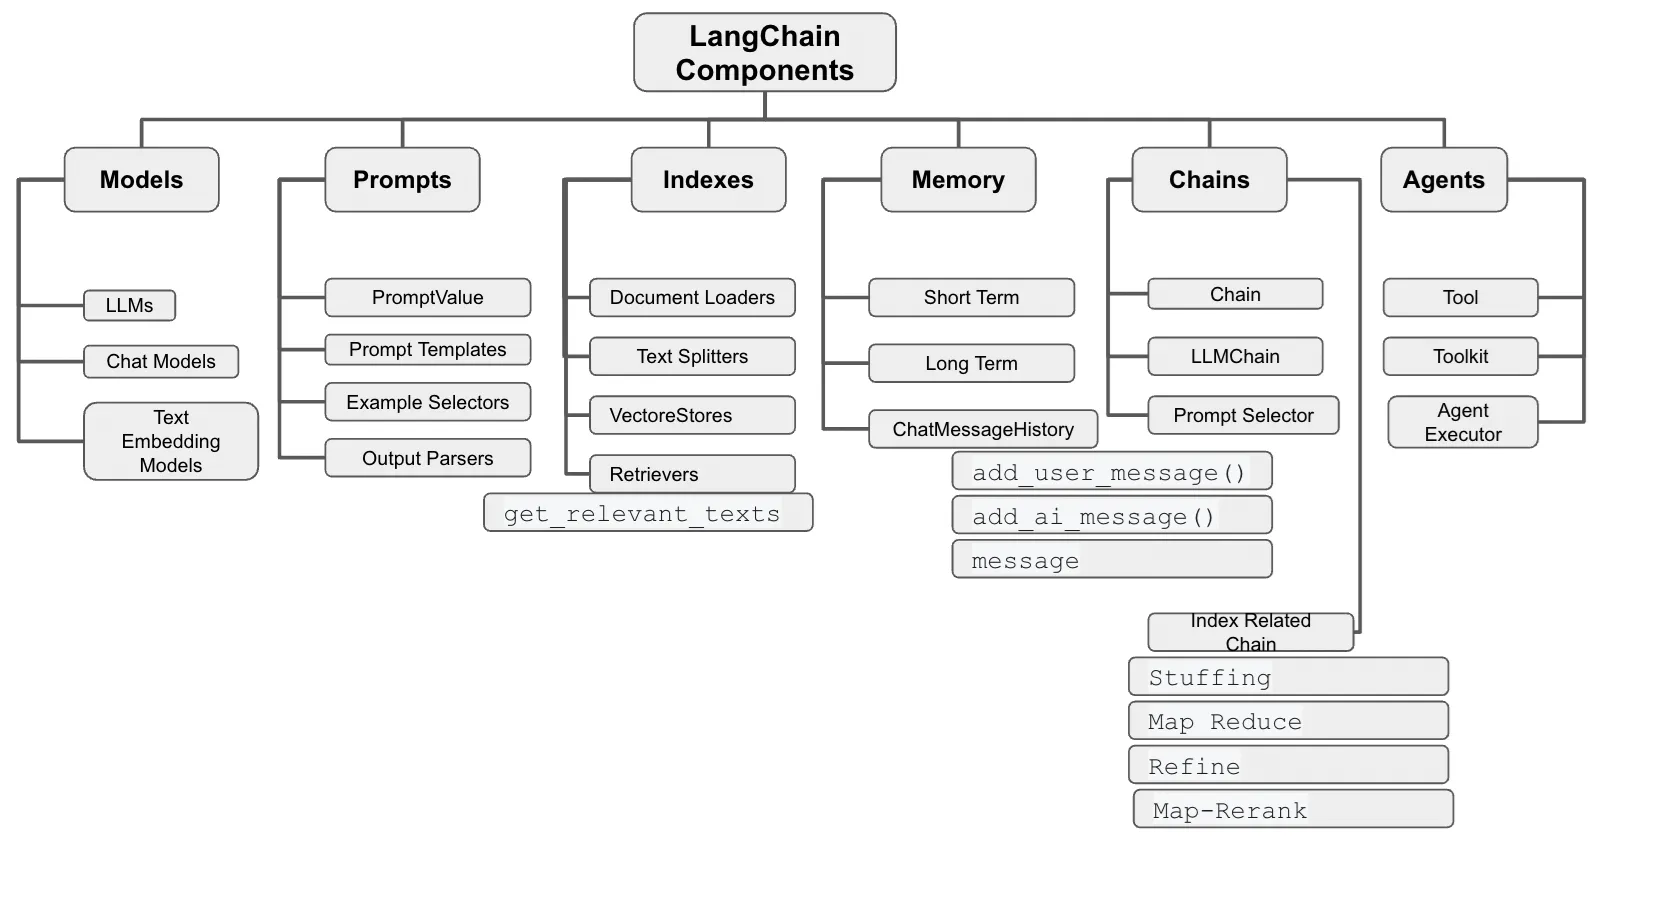
\includegraphics[width=\linewidth,keepaspectratio]{langchain16}
\end{center}	  


{\tiny (Ref: How LangChain Makes Large Language Models More Powerful: Part 2 -Renu Khandelwal)}



\end{frame}

%%%%%%%%%%%%%%%%%%%%%%%%%%%%%%%%%%%%%%%%%%%%%%%%%%%%%%%%%%%%%%%%%%%%%%%%%%%%%%%%%%
\begin{frame}[fragile]\frametitle{Models}

LangChain offers integration to a wide range of models and a streamlined interface to all of them. LangChain differentiates between three types of models that differ in their inputs and outputs:

\begin{itemize}
\item LLMs take a string as an input (prompt) and output a string (completion).
\item Chat models are similar to LLMs. They take a list of chat messages as input and return a chat message.
\item Text embedding models take text input and return a list of floats (embeddings), for calculating similarities between texts (e.g., movie summaries).
\item Proprietary Foundation Models, say, GPT from OpenAI and Gemini from Google 
\item Open Source models typically available at Hugging Face
\end{itemize}

\begin{center}
\includegraphics[width=0.5\linewidth,keepaspectratio]{langchain8}
\end{center}	  


{\tiny (Ref: LangChain 101: Part 1. Building Simple Q\&A App - Ivan Reznikov)}

\end{frame}

%%%%%%%%%%%%%%%%%%%%%%%%%%%%%%%%%%%%%%%%%%%%%%%%%%%%%%%%%%%%%%%%%%%%%%%%%%%%%%%%%%
\begin{frame}[fragile]\frametitle{Prompts}

  \begin{columns}
    \begin{column}{0.5\textwidth}
      \begin{itemize}
        \item \textbf{Definition}: Text guiding LLM for desired output.
        \item \textbf{Versatility}: Used for various tasks like text generation, translation, and Q\&A.
        \item \textbf{Critical in LangChain}: Essential for controlling LLM output.
        \item \textbf{Crafting Importance}: Influence LLM output through careful prompt crafting.
        \item \textbf{Output Format Specification}: Use prompts to instruct LLM for text generation, translation, or Q\&A.

      \end{itemize}
    \end{column}
    \begin{column}{0.5\textwidth}
			\begin{center}
			\includegraphics[width=\linewidth,keepaspectratio]{langchain9}
			\end{center}	  


			{\tiny (Ref: LangChain 101: Part 1. Building Simple Q\&A App - Ivan Reznikov)}
			
		
    \end{column}
  \end{columns}

\end{frame}


%%%%%%%%%%%%%%%%%%%%%%%%%%%%%%%%%%%%%%%%%%%%%%%%%%%%%%%%%%%%%%%%%%%%%%%%%%%%%%%%%%
\begin{frame}[fragile]\frametitle{Indexes}


      \begin{itemize}
        \item \textbf{Indexes}: Unique data structures for storing information about data.
        \item \textbf{Information Inclusion}: Terms, document locations, relationships, etc.
        \item \textbf{Vectorstores}: Data structures storing vector representations of dataset.
        \item \textbf{Retrievers}: Returning documents in response to unstructured queries.
        \item \textbf{Retriever vs. Vectorstore}: Retriever broader in scope than a vector store.
        \item \textbf{Key Components}: Understanding indexes, vectorstores, and retrievers.
        \item \textbf{App Development}: Essential for building apps on specific data.
        % \item \textbf{Example Chain Components}:
          % \begin{enumerate}
            % \item A chain for answering financial questions.
            % \item Index used to find documents with the word "finance."
            % \item Vectorstore locates terms similar to "finance" (e.g., ``money'').
            % \item Retriever retrieves top-ranked documents for the query "What are ways to invest?"
          % \end{enumerate}
      \end{itemize}

			\begin{center}
			\includegraphics[width=\linewidth,keepaspectratio]{langchain10}
			\end{center}	  


			{\tiny (Ref: LangChain 101: Part 1. Building Simple Q\&A App - Ivan Reznikov)}


\end{frame}

%%%%%%%%%%%%%%%%%%%%%%%%%%%%%%%%%%%%%%%%%%%%%%%%%%%%%%%%%%%%%%%%%%%%%%%%%%%%%%%%%%
\begin{frame}[fragile]\frametitle{Memory}

  % \begin{columns}
    % \begin{column}{0.5\textwidth}
      \begin{itemize}
	  \item By default, the Models are stateless meaning, for them, each query/prompt is independent, and it does not carry information from the past. But for applications like chatbot, remembering the context/session is important to have true conservation. Memory provides the requisite storage of the context.
        \item \textbf{Definition}: Method of storing data for LLM access.
        \item \textbf{Information Inclusion}: Previous chain results, current chain context, and other LLM-required data.
        \item \textbf{Context Retention}: Enables tracking of current conversation context.
        \item \textbf{Role in LangChain}: Vital for learning from previous interactions.
        \item \textbf{Knowledge Base Building}: Allows the LLM to build a knowledge base.
        \item \textbf{Performance Improvement}: Utilized to enhance future chain performance.
        % \item \textbf{Example Scenario}:
          % \begin{itemize}
            % \item Chain answering real estate-related questions.
            % \item Memory stores results of previous real estate-related chains.
            % \item Enhances performance when handling new questions on similar topics.
          % \end{itemize}
      \end{itemize}
    % \end{column}
    % \begin{column}{0.5\textwidth}
			\begin{center}
			\includegraphics[width=0.8\linewidth,keepaspectratio]{langchain11}
			\end{center}	  


			{\tiny (Ref: LangChain 101: Part 1. Building Simple Q\&A App - Ivan Reznikov)}
			
		
    % \end{column}
  % \end{columns}

\end{frame}

%%%%%%%%%%%%%%%%%%%%%%%%%%%%%%%%%%%%%%%%%%%%%%%%%%%%%%%%%%%%%%%%%%%%%%%%%%%%%%%%%%
\begin{frame}[fragile]\frametitle{Chains}

  % \begin{columns}
    % \begin{column}{0.5\textwidth}
      \begin{itemize}
	  \item One component is not sufficient for non-trivial applications. Need aggregation. One of the ways is, chaining.
        \item \textbf{Definition}: Sequences of instructions for task execution.
        \item \textbf{Connectivity}: Links various components based on requirements.
        \item \textbf{Versatility}: Enables a wide range of tasks within the framework.
        \item \textbf{Application Scenario}:
          \begin{enumerate}
            \item App for interview preparation.
            \item \textbf{Prompt}:``I'm getting ready for an interview \ldots ''

            \item \textbf{Function A}:
              \begin{itemize}
                \item Access LLM's knowledge in software engineering.
                \item Utilize vectorstore for relevant data.
              \end{itemize}
            \item \textbf{Function B}:
              \begin{itemize}
                \item Manipulate data: generate common interview questions.
                \item Prepare a list of resources for interview preparation.
                \item Select and ask a question.
              \end{itemize}
            \item \textbf{Memory Implementation}:
              \begin{itemize}
                \item Ask follow-up questions to understand chosen topic.
                \item Memory maintains conversation context.
              \end{itemize}
          \end{enumerate}
      \end{itemize}
    % \end{column}
    % \begin{column}{0.5\textwidth}
			\begin{center}
			\includegraphics[width=0.5\linewidth,keepaspectratio]{langchain12}
			\end{center}	  


			{\tiny (Ref: LangChain 101: Part 1. Building Simple Q\&A App - Ivan Reznikov)}
			
		
    % \end{column}
  % \end{columns}

\end{frame}

%%%%%%%%%%%%%%%%%%%%%%%%%%%%%%%%%%%%%%%%%%%%%%%%%%%%%%%%%%%%%%%%%%%%%%%%%%%%%%%%%%
\begin{frame}[fragile]\frametitle{Agents and Tools}

  % \begin{columns}
    % \begin{column}{0.5\textwidth}
      \begin{itemize}
        \item \textbf{Agents}: Uses LLM as a reasoning engine, can understand the query, decide the next course of action. They can be Action Agents (decides next steps, suitable for small tasks) or Plan-and-Execute Agents (decide the full action sequence, suitable for complex tasks).
        \item \textbf{Tools}: Function libraries aiding agent development. Assist in creating various agents for diverse tasks.
        \item \textbf{Importance in LangChain}:
          \begin{itemize}
            \item Agents perform specific tasks efficiently.
            \item Tools support development by providing function libraries.
          \end{itemize}
        \item \textbf{Examples}:
          \begin{itemize}
            \item \textbf{NewsGenerator Agent}: Generates news articles or headlines.
            \item \textbf{DataManipulator Tool}: Manipulates data (cleaning, transforming, extracting features).
          \end{itemize}
      \end{itemize}		  
    % \end{column}
    % \begin{column}{0.5\textwidth}
			\begin{center}
			\includegraphics[width=0.5\linewidth,keepaspectratio]{langchain13}
			\end{center}	  


			{\tiny (Ref: LangChain 101: Part 1. Building Simple Q\&A App - Ivan Reznikov)}
			
		
    % \end{column}
  % \end{columns}

\end{frame}

%%%%%%%%%%%%%%%%%%%%%%%%%%%%%%%%%%%%%%%%%%%%%%%%%%%%%%%%%%%%%%%%%%%%%%%%%%%%%%%%%%
\begin{frame}\frametitle{Why LangChain?}

\begin{itemize}
\item LLMs and Prompts: Prompt management, Prompt optimization, Generic interface for all LLMs and Common utilities for working with LLMs. Powers the agent.
\item Chains: Chains are sequences of calls that whether to an LLM or a different utility. LangChain provides a standard interface for chains, many integrations with other tools, \& end-to-end chains for common applications. Chains go in order.
\item External Data Augmentation: Specific types of chains that first interact with an external data source to fetch data to use in the generation step. Examples of this include summarization of long pieces of text \& question/answering over specific data sources
\item Agents: Agents involve an LLM making decisions about which actions to take, taking that action, seeing an observation, \& repeating that until done. LangChain provides a standard interface for agents, a selection of agents to choose from, and examples of end-to-end agents. Agents decide the next action based on LLM response. Agents are entities that drive decision-making in LangChain. They have access to a suite of tools and can decide which tool to call based on user input. 
\end{itemize}

{\tiny (Ref: Linkedin Post by Munjal Patel)}
\end{frame}


%%%%%%%%%%%%%%%%%%%%%%%%%%%%%%%%%%%%%%%%%%%%%%%%%%%%%%%%%%%%%%%%%%%%%%%%%%%%%%%%%%
\begin{frame}\frametitle{Why LangChain?}

\begin{itemize}
\item Toolkits are sets of tools that, when used together, can accomplish a specific task. The Agent Executor is responsible for running agents with the appropriate tools.
\item Tool: A function that performs a specific duty. This can be things like: Google Search, Database lookup,
\item Memory: Memory refers to the concept of persisting state between calls of a chain/agent. LangChain provides a standard interface for memory, a collection of memory implementations, and examples of chains/agents that use memory.
\item Evaluation [BETA]: Generative models are notoriously hard to evaluate with traditional metrics. One new way of evaluating them is using language models themselves to do the evaluation. LangChain provides some prompts/chains for assisting in this.
\end{itemize}

{\tiny (Ref: Linkedin Post by Munjal Patel)}
\end{frame}


%%%%%%%%%%%%%%%%%%%%%%%%%%%%%%%%%%%%%%%%%%%%%%%%%%%%%%%%%%%%%%%%%%%%%%%%%%%%%%%%%%
\begin{frame}[fragile]\frametitle{}
\begin{center}
{\Large Sample Implementations}
\end{center}
\end{frame}

%%%%%%%%%%%%%%%%%%%%%%%%%%%%%%%%%%%%%%%%%%%%%%%%%%%%%%%%%%%%%%%%%%%%%%%%%%%%%%%%%%
\begin{frame}[fragile]\frametitle{Hugging Face}

\begin{lstlisting}
from langchain import HuggingFaceHub
llm = HuggingFaceHub(repo_id = "google/flan-t5-xl")

# The LLM takes a prompt as an input and outputs a completion
prompt = "Alice has a parrot. What animal is Alice's pet?"
completion = llm(prompt)

from langchain.embeddings import HuggingFaceEmbeddings
embeddings = HuggingFaceEmbeddings(model_name = "sentence-transformers/all-MiniLM-L6-v2")

# The embeddings model takes a text as an input and outputs a list of floats
text = "Alice has a parrot. What animal is Alice's pet?"
text_embedding = embeddings.embed_query(text)


\end{lstlisting}


\end{frame}

%%%%%%%%%%%%%%%%%%%%%%%%%%%%%%%%%%%%%%%%%%%%%%%%%%%%%%%%%%%%%%%%%%%%%%%%%%%%%%%%%%
\begin{frame}[fragile]\frametitle{Gen AI Google}

Prerequisites
\begin{itemize}
\item Select or create a Google Cloud project.
\item Make sure that billing is enabled for your project.
\item Enable the Vertex AI API
\item Create credentials json (Ref https://www.youtube.com/watch?v=rWcLDax-VmM)
\item Set Environment variable GOOGLE\_APPLICATION\_CREDENTIALS as the above created json
\item Create conda environment with \lstinline|python=3.10 (?)|
\item Activating that environment, \lstinline|pip install google-cloud-aiplatform==1.27|
\item Install langchain
\end{itemize}


\end{frame}


%%%%%%%%%%%%%%%%%%%%%%%%%%%%%%%%%%%%%%%%%%%%%%%%%%%%%%%%%%%%%%%%%%%%%%%%%%%%%%%%%%
\begin{frame}[fragile]\frametitle{Gen AI Google}

% Ref https://python.langchain.com/docs/modules/model\_io/models/llms/integrations/google\_vertex\_ai\_palm

\begin{lstlisting}
from langchain.llms import VertexAI
from langchain import PromptTemplate, LLMChain

template = """Question: {question}
Answer: Let's think step by step."""

prompt = PromptTemplate(template=template, input_variables=["question"])
llm = VertexAI()
llm_chain = LLMChain(prompt=prompt, llm=llm)
question = "What NFL team won the Super Bowl in the year Justin Beiber was born?"
response = llm_chain.run(question)
print(response)

llm = VertexAI(model_name="code-bison")
llm_chain = LLMChain(prompt=prompt, llm=llm)
question = "Write a python function that identifies if the number is a prime number?"
response = llm_chain.run(question)
print(response)
\end{lstlisting}


\end{frame}




%%%%%%%%%%%%%%%%%%%%%%%%%%%%%%%%%%%%%%%%%%%%%%%%%%%%%%%%%%%%%%%%%%%%%%%%%%%%%%%%%%
\begin{frame}[fragile]\frametitle{Clarifications}

\begin{itemize}
\item A chain is a sequence of components (or other chains) put together to accomplish a specific task. For example, a chain might include a prompt template, a language model, and an output parser, all working together to handle user input, generate a response, and process the output.
\item Chains vs Agents: Whereas a chain defines an immediate input/output process, the logic of agents allows a step-by-step thought process. The advantage of this step-by-step process is that the LLM can work through multiple reasoning steps or tools to produce a better answer.
\item Generic chains as standalone chains are used rarely. There are specialized chains, comprised of many LLMs to help solve a specific task. For example, LangChain supports some end-to-end chains (such as AnalyzeDocumentChain for summarization, QnA, etc) and some specific ones (such as GraphQnAChain for creating, querying, and saving graphs). 
\item Chains can be composed of entities other than LLMs, say, chaining agents and LLMs together.
\end{itemize}

{\tiny (Ref: 'Superpower LLMs with Conversational Agents', 'A Gentle Intro to Chaining LLMs, Agents, and utils via LangChain', etc)}
\end{frame}

%%%%%%%%%%%%%%%%%%%%%%%%%%%%%%%%%%%%%%%%%%%%%%%%%%%%%%%%%%%%%%%%%%%%%%%%%%%%%%%%%%
\begin{frame}[fragile]\frametitle{Clarifications}

\begin{itemize}
\item An agent has access to an LLM to parse the input query and decide the tool to be used and a suite of tools for example Google Search, Python REPL, math calculator, weather APIs, etc. to do the actual work.
\item What’s the point of getting an agent to do the same thing that an LLM can do. Some applications will require not just a predetermined chain of calls to LLMs/other tools, but potentially an unknown chain that depends on the user’s input. In these types of chains, there is an 'agent' which has access to a suite of tools e.g. an agent that can fetch the correct documents (from the vectorstores) for RetrievalQAChain depending on whether the question refers to document A or document B.
\end{itemize}

{\tiny (Ref: 'Superpower LLMs with Conversational Agents', 'A Gentle Intro to Chaining LLMs, Agents, and utils via LangChain', etc)}
\end{frame}

%%%%%%%%%%%%%%%%%%%%%%%%%%%%%%%%%%%%%%%%%%%%%%%%%%%%%%%%%%%%%%%%%%%%%%%%%%%%%%%%%%
\begin{frame}[fragile]\frametitle{Clarifications}

Combine Agent and Chain in another chain.

\begin{lstlisting}
# Chain1 - solve math problem, get the age
chain_one = agent

# Chain2 - suggest age-appropriate gift
template = """You are a gift recommender. Given a person's age,\n
 it is your job to suggest an appropriate gift for them.

Person Age:
{age}
Suggest gift:"""
prompt_template = PromptTemplate(input_variables=["age"], template=template)
chain_two = LLMChain(llm=llm, prompt=prompt_template) 

from langchain.chains import SimpleSequentialChain

overall_chain = SimpleSequentialChain(
                  chains=[chain_one, chain_two],
                  verbose=True)
				  
question = "If my age is half of my dad's age and he is going to be 60 next year, what is my current age?"
overall_chain.run(question)				  
\end{lstlisting}

\end{frame}


%%%%%%%%%%%%%%%%%%%%%%%%%%%%%%%%%%%%%%%%%%%%%%%%%%%%%%%%%%%%%%%%%%%%%%%%%%%%%%%%%%
\begin{frame}\frametitle{LangChain Usecases}

\begin{itemize}
\item Personal assistants
\item Question answering over database(s)
\item Chatbots
\item Querying tabular data
\item Interacting with APIs
\item Model Evaluation
\end{itemize}


{\tiny (Ref: Linkedin Post by Munjal Patel)}
\end{frame}


%%%%%%%%%%%%%%%%%%%%%%%%%%%%%%%%%%%%%%%%%%%%%%%%%%%%%%%%%%%%%%%%%%%%%%%%%%%%%%%%%%
\begin{frame}\frametitle{How LangChain Works?}

\begin{itemize}
\item Text is preprocessed by breaking it down into chunks or summaries, 
\item embedding them in a vector space, 
\item searching for similar chunks when a question is asked. 
\end{itemize}

\begin{center}
\includegraphics[width=0.5\linewidth,keepaspectratio]{langchain4}
\end{center}	  


{\tiny (Ref: Getting started with LangChain - Avra)}
\end{frame}

%%%%%%%%%%%%%%%%%%%%%%%%%%%%%%%%%%%%%%%%%%%%%%%%%%%%%%%%%%%%%%%%%%%%%%%%%%%%%%%%%%
\begin{frame}[fragile]\frametitle{LangChain Setup}

\begin{lstlisting}
pip install langchain openai cohere huggingface_hub \
ipywidgets chromadb google-search-results

import os
import langchain
from langchain.llms import OpenAI, Cohere, HuggingFaceHub
from langchain.chat_models import ChatOpenAI
from langchain.schema import (
    AIMessage,
    HumanMessage,
    SystemMessage
)
os.environ["OPENAI_API_KEY"] = ""
os.environ["COHERE_API_KEY"] = ""
os.environ["HUGGINGFACEHUB_API_TOKEN"] = ""
os.environ["SERPAPI_API_KEY"] = ""
\end{lstlisting}	  

\end{frame}

%%%%%%%%%%%%%%%%%%%%%%%%%%%%%%%%%%%%%%%%%%%%%%%%%%%%%%%%%%%%%%%%%%%%%%%%%%%%%%%%%%
\begin{frame}[fragile]\frametitle{LangChain Integration}

\begin{lstlisting}
chatgpt = ChatOpenAI(model_name='gpt-3.5-turbo')
gpt3 = OpenAI(model_name='text-davinci-003')
cohere = Cohere(model='command-xlarge')
flan = HuggingFaceHub(repo_id="google/flan-t5-xl")

text = "How to be happy?"

print(chatgpt([HumanMessage(content=text)]))
print(gpt3(text))
print(cohere(text))
print(flan(text))
\end{lstlisting}	  

\end{frame}
